\documentclass{llncs}
\usepackage{epsf}
\usepackage{graphicx}

\begin{document}

\title{Predictive Text Entry of Agglutinative Languages using Morphological Segmentation and Phonological Restrictions}

\author{\ldots}
\institute{\ldots}

\maketitle

\begin{abstract}

Linguistic models for predictive text entry on ambiguous keyboards
typically rely on large dictionaries including word frequenies, which
are used to disambiguate between words matching user input. This
approach is insufficient for heavily agglutinative languages, like
Finnish or Turkish, where morphological phenomena such as inflection
and compounding increase the rate of out-of-vocabulary words. We
propose a method for text entry, which circumvents the problem of
out-of-vocabulary words, by replacing the dictionary with a Markov
chain on morpheme sequences constructed from morphologically segmented
training data. The Markov chain is combined with a third order hidden
Markov model (HMM) mapping key sequences to letter
sequences. Additionally we use rules, which enforce phonotactic
restrictions such as vowel harmony in Finnish. We evaluate our method
by constructing text entry systems for Finnish and Turkish mobile
phone keypads. We compare the Turkish text entry system with an
existing system, which is based on an HMM of letter sequences
\cite{Tantug:2010} and show that we achieve superior results measured
by the keystrokes per character ratio (KPC)
\cite{MacKenzie02kspc}. We also compare the Finnish text entry system
to an existing system, which utilizes a morphological analyzer
combined with a colloquial dictionary \cite{silfverberg/2011/cla} and
show that we achieve superior KPC. For segmenting the training data,
we use Morfessor, a system for unsupervised morphological segmentation
\cite{Creutz07ACMTSLP}. For constructing the probabilistic models
needed for the text entry systems, we use tools for POS tagging from
the HFST interface \cite{Silfverberg/2011}, which is an open-source
interface for weighted finite-state calculus. We also utilize an
open-source two-level phonology rule compiler, hfst-twolc, for
implementing the vowel harmony rules needed for text entry of Finnish
\cite{hfst/2011}.

\end{abstract}

\section{Introduction}

\section{Earlier Approaches to Predictive Text Entry}

\section{A Probabilistic Model of Word Structure}

\subsection{An Hidden Markov Model for Predicting Letter Sequences from Key Sequences}

\subsection{A Markov Chain of Morphs}

\subsection{Phonological Constraints}

\subsection{Combining Models using Weighted Finite-State Calculus}

\section{Training Materials and Test Materials for Finnish and Turkish}

\subsection{Finnish}

\subsection{Turkish}

\section{Evaluation}

Many factors influence the efficiency of mobile phone text entry in
practice. E.g. the general user interface design of the phone and
specifically the design of the keyboard have a large
impact. Nevertheless such factors are in some sense isolated from the
predicitve text entry algorithm itself, which makes it plausible to
evaluate the algorithms in isolation from the rest of the user
interface of mobile phones. In this paper we use the keystrokes per
character (KPC) ratio~\cite{MacKenzie02kspc} for measuring the efficiency of text entry. It
measures the average number of keystrokes required to input one letter
in a text message.


\subsection{The Keystrokes Per Characters Ratio}



\begin{figure}[hbt]
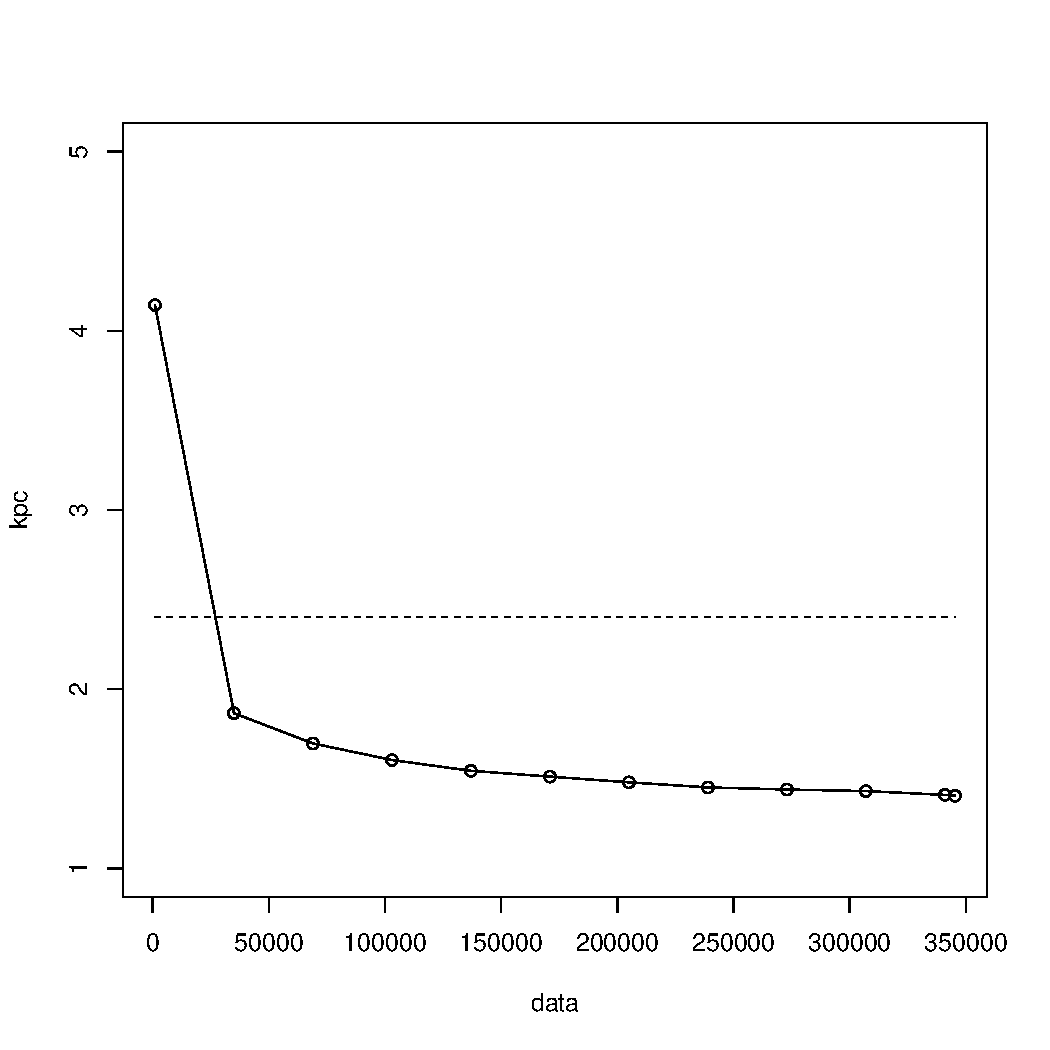
\includegraphics[width=4in]{finnish_kpc_figure.pdf}
\end{figure}

\section{Discussion}

\section{Conclusions}

\section{Acknowledgments}

\bibliographystyle{splncs03}
\bibliography{cicling2011.bib}
\end{document}
